\chapter{Préparation des données}

Ce projet nous a confrontés à plusieurs types de problèmes de données auxquels il a fallu trouver une solution ou faire un choix.

Parmi les données à problème, il y en avait trois types~:
\begin{itemize}
    \item les informations volontairement mauvaises et aberrantes, insérées par une personne bienveillante soucieuse de nous inciter à porter un regard critique sur le jeu de données qui nous a été confié~;
    \item les données particulières de type "Chine" qui perturbent les échelles en constituant des clusters très à part des autres~;
    \item les données involontairement aberrantes ou incomplètes insérées par les utilisateurs et transmises sous des formats variés.
\end{itemize}
\vspace{5mm}

\begin{figure}[!h]
    \centering
    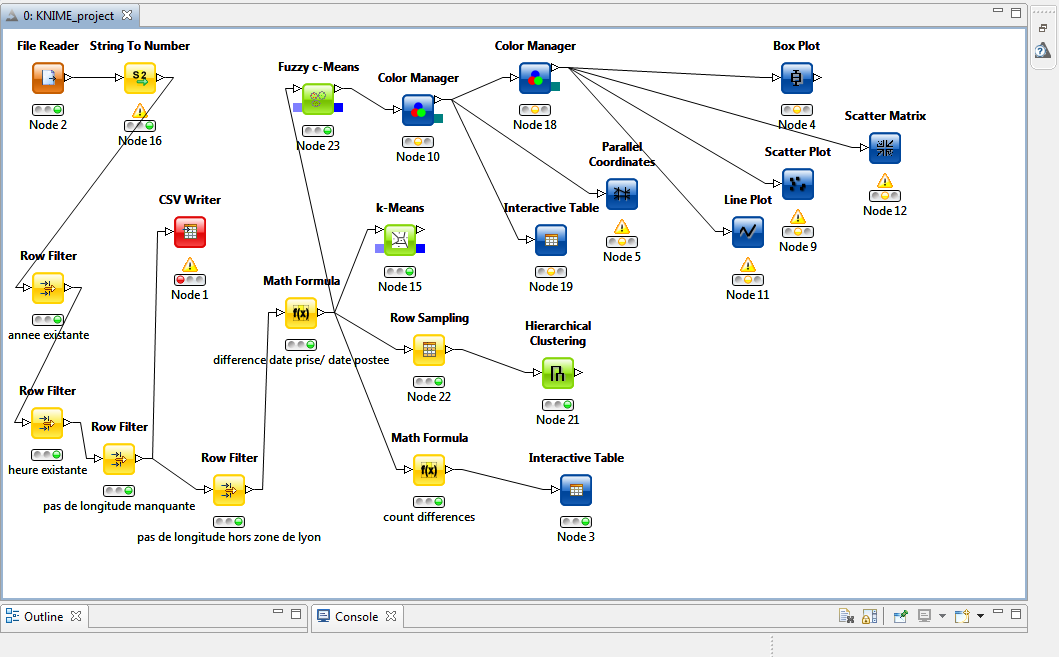
\includegraphics[width=14cm]{images/captureKnime.png}
    \caption{Apercu de la préanalayse et de la préparation des données sous knime}
    \label{fig:knime}
\end{figure}

\section{Lecture du fichier sur Knime}
Avant même de pouvoir commencer à regarder les données sur Knime pour faire une première préparation, il a fallu nettoyer les données de manière inattendue. En effet, les données commençant par des balises HTML entrainaient un plantage de la lecture du fichier pour Knime. Il a donc fallu encadrer de guillemets sur le même modèle que d'autres lignes fonctionnelles, les balises fautives.

\section{Les informations «~troll~»}
Nous avons fait le choix d'écarter sans remord les données appartenant à ce type.
Il s'agissait de données où les dates et heures de prise ou d'upload de photos étaient impossibles (par exemple, le 89\up{ème} jour du mois, ou encore avant l'invention de la photographie), mais aussi une ligne qui ne possédait ni longitude ni latitude.
Ces lignes volontairement aberrantes étaient pour la plupart facilement identifiables comme des lignes «~trolls~», et non comme des erreurs utilisateur, grâce aux légendes et tags qui les composaient.

\section{Les données particulières}
Une donnée a particulièrement été repérée comme étant à l'écart des autres. Il s'agissait d'une photo prise en latitude et longitude 0. Ne sachant pas si cette ligne s'inscrivait dans la série des aberrations insérées volontairement ou s'il s'agissait d'une photo du véritable jeu de données, nous l'avons sérieusement considérée et c'est pourquoi elle est évoquée dans cette catégorie à part.
Nous avons néanmoins fait le choix d'écarter cette ligne tout comme les informations troll car elle perturbait à la fois les calculs de clusters, mais aussi les échelles, tant sous Knime pour la pré-analyse, que sous Google Map lors de l'affichage des clusters trouvés.

D'autres données auraient pu nous perturber si nous avions essayé de clusteriser en fonction de mots présents dans les tags ou les légendes, car certains d'entre eux ont été écrits dans des langues n'utilisant pas les caractères latins (chinois, japonnais, arabe, etc.), ces lignes auraient pu générer des erreurs si nous avions tenté d'analyser leur contenu textuel. Puisque nous n'avons pas eu le temps d'étudier les textes pour clusteriser, car cela aurait demandé une base de connaissance des synonymes au moins en français, nous avons laissé les lignes en langues étrangères.

\section{Les mauvaises informations utilisateur}
Enfin, les problèmes les plus importants viennent des informations ou justement du manque d'information utilisateur.

Il aurait difficile de clusteriser les éléments textuels car tous les utilisateur ne taggent ou ne légendent pas leurs photos. De plus, au sein des textes, il n'est pas dit que les utilisateur parlent le même vocabulaire ou du même intérêt pour évoquer un lieu. Et quand bien même le feraient-ils, resterait encore le problème de gérer les fautes d'orthographe qui créent de nouveaux mots ou l'importance des majuscules/minuscules dans la comparaison de deux mots.

De plus un phénomène étrange a été observé sur environ 70 photos. Celles-ci auraient été uploadées avant même d'être prises. Même si l'erreur semble au premier abord être une information «~troll~» insérée artificiellement, elle se reproduit suffisamment pour pouvoir être considérée comme un comportement utilisateur atypique mais acceptable.
Dans la mesure où ce comportement ne perturbait pas le calcul des clusters, nous avons choisi de le tolérer dans le jeu de données.

